\documentclass[11pt,dvipdfmx]{jreport}
\usepackage{wuse_thesis}
\usepackage{indentfirst}
\usepackage{url}	% \url{}コマンド用.URLを表示する際に便利
\usepackage{graphicx}  % ←graphicx.styを用いてEPSを取り込む場合有効にする
\usepackage{listings}
\usepackage{multirow}

\usepackage{color}

\renewcommand{\lstlistingname}{Program}
\newcommand{\todo}[1]{\colorbox{yellow}{{\bf TODO}:}{\color{red} {\textbf{[#1]}}}}
			% 他のパッケージ・スタイルを使う場合には適宜追加

%%%%%%%%%%%%%%%%%%%%%%%%%%%%%%%%%%%%%%%%%%%%%%%%%%%%%%%%%%%%%%%%%%%%%%%%

%%
%% 主に表紙を作成するための情報
%%

%%  タイトル(修論の場合は英語表記も指定)
\title{JavaScriptテストコード変更内容に基づく\\後方互換性損失の検出}
%\etitle{Test\\Test\\Test}

%%  著者名(修論の場合は英語表記も指定)
\author{前川 大樹}
%\eauthor{Akinori Ihara}

%% 卒業論文・修士論文(以下のどちらかを選択)
\bachelar	% 卒業論文(4年生用)
%\master  	% 修士論文(M2用)

%%  学科・クラスタ
\department{システム工}
%\department{デザイン情報}
%\department{デザイン科学}

%%  学生番号
\studentid{60256245}

%%  卒業年度
\gyear{2023}		% 提出年が2022年なら,2021年度

%%  論文提出日
\date{2024年2月13日}	% 修士の場合は月(2021年2月)までとし,英語表記も指定
%\edate{February 2021}	% 修士の場合,こちら(英語表記)も有効化

%%%%%%%%%%%%%%%%%%%%%%%%%%%%%%%%%%%%%%%%%%%%%%%%%%%%%%%%%%%%%%%%%%%%%%%%

\begin{document}

\maketitle

%%
%%  概要
%%
\begin{abstract}
  ソフトウェア開発では,ライブラリと呼ばれる再利用可能なプログラムの利用により,開発者自身が同じ機能を再実装する必要がなくなり開発効率が向上する.ライブラリは機能追加やバグ修正により頻繁に更新されているため,利用者は適宜ライブラリの更新を適用する必要がある.利用者がライブラリの更新を自身のソフトウェアに適用する際,利用者のソフトウェアが期待通りに動作しなくなることがある.このような,更新後のライブラリが利用者のソフトウェアに影響を与えることを後方互換性の損失という.ライブラリ開発者は,利用者が安全にライブラリ更新を適用できるように,後方互換性の損失を利用者に正確に伝える必要があるが,後方互換性を正確に判定することは困難である.従来研究では,ライブラリの動作を検証するテストコードの変更有無に着目した後方互換性の判定手法を提案している.しかし,テストコードの変更内容は考慮されておらず,誤検出も多い.そこで本研究では,テストコードの変更内容を考慮した後方互換性の判定手法を提案し,その精度を検証する.その結果\todo{結果}

\end{abstract}

%%  目次
\tableofcontents

%%  図目次 (図目次をいれたければ以下のコメントをはずす)
%\listoffigures

%%  表目次 (表目次をいれたければ以下のコメントをはずす)
%\listoftables

\newpage
\pagenumbering{arabic}	% 以降のページ番号を算用数字に

%%%%%%%%%%%%%%%%%%%%%%%%%%%%%%%%%%%%%%%%%%%%%%%%%%%%%%%%%%%%%%%%%%%%%%%%

%%
%%  本文はここから
%%

\chapter{はじめに}
ソフトウェア開発では,ライブラリと呼ばれる再利用可能なプログラムの利用により,開発者自身が同じ機能を再実装する必要がなくなり開発効率が向上する.ライブラリは機能追加やバグ修正により頻繁に更新されており,利用者は適宜ライブラリのバージョン更新が必要である.利用者が安全にライブラリを更新するために,パッケージマネージャはセマンティックバージョニング\footnote{\url{https://semver.org}}を採用し,バージョン間の互換性の有無を管理している.セマンティックバージョニングでは,ライブラリ更新をメジャー,マイナー,パッチのレベルに分類し,マイナーとパッチの更新では後方互換性を保つ変更が求められる.しかし,バージョン名の付与は開発者が手動で行うため,後方互換性が損失しているにも関わらず,誤ってマイナーやパッチに分類されてしまうことがある.
この問題は,特にJavaScriptのような動的な言語において顕著であり,ライブラリと利用者のコードの不整合が実行時まで検出されないという課題がある.
この課題に対して,JavaScriptライブラリの後方互換性を判定する研究が行われている.

松田らは,後方互換性を損失するライブラリの更新は,プログラムの更新と合わせてテストコードも修正すると考え,テストコードの変更有無による後方互換性の判定手法を提案した.
\cite{matsuda}
しかし,テストコードの変更内容を考慮しておらず,テストの誤り修正や実行手順の修正など,ライブラリ変更とは無関係のテストコード変更についても後方互換性を損失したと誤検出する.

本研究では,テストコードの変更内容に着目し,後方互換性の損失に関係するテスト変更内容を明らかにし,テスト変更内容に基づく後方互換性の判定手法の精度を評価する.具体的には,2つのリサーチクエスチョン(RQ)に回答する.

\begin{itemize}
  \item RQ1:後方互換性の損失に関係するテストコード変更とは何か?
  \item RQ2:テストコード変更内容に基づく後方互換性の判定手法の有効性はどの程度か?
\end{itemize}

\chapter{後方互換性の損失}

\section{クライアントへの影響}
ライブラリの後方互換性の損失とは,ライブラリのバージョン更新によって,更新前のバージョンとの互換性が損なわれることを指す.クライアントソフトウェアは,更新前のライブラリ仕様を前提とするため,後方互換性を損失するライブラリのバージョン更新を適用する際,コードの不整合によるエラーが起きることがある.この問題に対して,ライブラリ開発者は後方互換性の損失を含むライブラリ更新をクライアントに正確に伝えることが求められる.

ライブラリ開発者がクライアントに後方互換性の損失を伝える手法として,セマンティックバージョニング\footnote{\url{https://semver.org}}がある.セマンティックバージョニングは,バージョン名を付与するための規則でバージョン名はそのソフトウェアの変更点や互換性に関する情報を提供する.バージョン名は,{\verb|MAJOR.MINOR.PATCH|}の形式をとる.後方互換性を損失する変更では{\verb|MAJOR|},後方互換性を保つ変更では{\verb|MINOR|}または{\verb|PATCH|}の値を増やすことで後方互換性の有無をクライアントに伝える.

ライブラリ更新をメジャー,マイナー,パッチのレベルに分類し,バージョン名によって後方互換性の有無を,後方互換性を損失する変更ではメジャーを,後方互換性を保つ変更ではマイナーバージョンもしくはパッチバージョンを更新する.しかし,バージョン名の付与はライブラリ開発者が手動で行うため,後方互換性が損失しているにも関わらず誤ってマイナーやパッチに分類されてしまうことがある.



\section{後方互換性の損失の原因}
クライアントソフトウェアの開発者が依存ライブラリのバージョン更新を取り込む際,クライアントは更新前のライブラリ仕様を前提とするため不整合によるエラーが起きることがある.この問題に対して,ライブラリ開発者は利用者に影響があるライブラリ変更を意図せずバージョン更新に含めないことが求められる.

ライブラリ開発者によって新しいライブラリバージョンがリリースされた際,更新前のライブラリ仕様を前提としたクライアントソフトウェアとの不整合が起きることがある.

更新前のライブラリ仕様を前提としたクライアントと,更新後の


ライブラリの後方互換性の損失とは,新しいバージョンのライブラリがリリースされた際に,以前のバージョンとの互換性が損なわれることを指す.後方互換性を損失する更新が入ったライブラリバージョンをクライアントソフトウェアが適用すると,クライアントソフトウェアが期待通りに動作しなくなることがあるため,ライブラリ開発者は意図せず後方互換性を損失する変更をバージョン更新に含めないことが求められる.

\section{関連研究}

\subsection{ライブラリ変更に基づく後方互換性の検出手法}

\subsection{テストケースに基づく後方互換性の検出手法}

\section{キーアイデア}

\chapter{RQ1:後方互換性の損失に伴うテストコード変更とは何か?}\label{rq1}

\section{概要}
本章では,実際に後方互換性が損失した時,どのようなテスト変更が行われているか分析する.具体的には,テストコード変更内容を定義し,各ライブラリバージョンに対して,テストコード変更内容ごとに後方互換性の有無を集計する.各バージョンのテストコードの変更内容はテストコードの変更差分から目視により分類する.実際の後方互換性の判定はMujahidらの手法を使用する.

% 後方互換性が損失しているかの判断基準は,従来研究のものを採用する.

% 本章では,テストコード変更内容を分類し,実際に後方互換性が損失する時どのようなテストコード変更が行われるかを明らかにする.テストコード変更内容を分類するために,まず,JavaScript言語におけるテストコードの構成要素を定義し,テストコード変更内容の細分化を行う.その後,目視によりバージョン間のテストコード変更内容を集計する.

\section{分析手法}
本分析では,各ライブラリ更新ごとにテストコード変更内容を目視により分類し,後方互換性を判定する.後方互換性の判定結果はテストコード変更内容ごとに集計する.

\subsection{テストコード変更内容の目視分類}
テストコード変更内容を定義するにあたり,テストコードの構成要素をまとめる.本研究では,プログラムのテストの中でも単体テストを対象とする.単体テストとは,関数やクラスといったプログラムを構成する単位(ユニット)が開発者の想定通りに動作するかを検証するテスト手法である.単体テストを実施する際は,テスト対象ユニットに対応するテストスイートを用意することが多い.テストスイートとは,テストの目的や条件が似ているテストケースの集合を指す.テストケースとは,テスト項目の最小単位であり,テスト対象への入力と想定される結果(期待値)の組み合わせで構成される.入力値と期待値を受け取ってプログラムが正しく動作しているか検証する仕組みをアサーションと呼ぶ.

JavaScriptにおけるテストコードの例をProgram~\ref{isOdd.js},Program~\ref{isOdd.test.js}を用いて説明する.Program~\ref{isOdd.js}は,この例においてテスト対象となる関数{\verb|isOdd()|}が定義されている.{\verb|isOdd()|}は,入力された値が奇数かどうかを真偽値で返す関数である.Program~\ref{isOdd.test.js}は,関数{\verb|isOdd()|}を単体テストによって検証するファイルで,JavaScript向けテストフレームワークJest\footnote{\url{https://jestjs.io/}}を使用して記述されている.JavaScript言語では,テストコードを書く際にフレームワークを使用することが多いが,フレームワーク毎に記法は異なるものの構成要素は変わらない.

Program~\ref{isOdd.test.js}に含まれる{\verb|describe|}関数でテストスイートを宣言し,{\verb|test|}関数により2つのテストケースが定義されている.テストスイートをネストさせることも可能である.テストスイートやテストケースは,そのテストスイート・ケースで何を検証するかが記述されるラベルと,検証するテスト用関数を引数に取る.1つ目のテストケースでは,5行目のアサーションにより,関数{\verb|isOdd()|}に対し正の奇数を入力したときの動作を検証している.この場合,想定結果は{\verb|true|}となるため,{\verb|toBe|}節で結果が{\verb|true|}となることを主張する.
同様に,2つ目のテストケースでは,関数{\verb|isOdd()|}に対し正の偶数を入力したときの動作を検証しており,想定結果は{\verb|false|}となるため{\verb|toBe|}節で結果が{\verb|false|}となることを主張している.

\begin{figure}[t]
  \begin{lstlisting}[caption={[upper/lower text]%
    \begin{tabular}[t]{@{}l@{}}
      isOdd.js \\[1.0\normalbaselineskip]
    \end{tabular}}, frame={tb}, numbers=left, label=isOdd.js, identifierstyle={\small}]
export function isOdd(number) {
  let result = false;
  if (number % 2 === 1) {
    result = true;
  }
  return result;
}
  \end{lstlisting}
  \vspace{-6mm}
\end{figure}


\begin{figure}[t]
  \begin{lstlisting}[caption={[upper/lower text]%
    \begin{tabular}[t]{@{}l@{}}
      isOdd.test.js \\[1.0\normalbaselineskip]
    \end{tabular}}, frame={tb}, numbers=left, label=isOdd.test.js, identifierstyle={\small}]
import { isOdd } from './isOdd';

describe('Testing the isOdd function', function() {
  test('should return true, if the number is odd', function() {
    expect(isOdd(3)).toBe(true);
  });
  test('should return false, if the number is even', function() {
    expect(isOdd(2)).toBe(false);
  });
});
  \end{lstlisting}
  \vspace{-6mm}
\end{figure}

% \begin{itemize}
%   \setlength{\itemsep}{0cm}
%   \item テストスイート(3から0行目)
%   \item テストケース(4から6行目,7から9行目)
%   \item テストスイート・テストケースのラベル(3,4,7行目)
%   \item アサーション(5,8行目)
%   \item 入力値(5,8行目{\verb|expect|}節の引数)
%   \item 期待値(5,8行目{\verb|toBe|}節の引数)
% \end{itemize}

また,テストデータの初期化や外部リソースの準備などは,セットアップ関数に記載したり,テストケース内に書くことができる.これらはテストケースの前提条件として扱う.また,その他の変更として,テストスイート・テストケースのラベルの変更,テストフレームワークの変更,可読性向上のためのフォーマッティングなどが挙げられるが,これらはテストコードの振る舞いに関わらない変更のためリファクタリングとして扱う.以上を踏まえ,本論文では,テストコードの変更内容として10件の内容を考慮する.

\begin{itemize}
  \setlength{\itemsep}{0cm}
  \item テストスイートの追加
  \item テストスイートの削除
  \item テストケースの追加
  \item テストケースの削除
  \item アサーションの追加
  \item アサーションの削除
  \item アサーションの入力値の変更
  \item アサーションの期待値の変更
  \item テストケースの前提条件の変更
  \item リファクタリング
\end{itemize}

\subsection{実際の後方互換性の判定}\label{zissainokouhougokanseinohantei}
実際の後方互換性の判定には,Mujahidらの手法を使用する.Mujahidらは,ライブラリの後方互換性の損失をクライアントテストを実行することで検出する手法を提案した\cite{mujahid}.後方互換性を損失する変更を加えられたライブラリバージョンでは,その影響を受けるクライアントテストの結果が更新前後で成功から失敗に変化することを手法の根拠としている.本分析でも,後方互換性の判定のためにクライアントテストを実行する.

\section{データセット}
データセットとして,従来研究\cite{matsuda}で収集されたライブラリバージョン群を使用する.従来研究では,人気でテストを継続的に管理しているライブラリを対象とするため,ライブラリの人気度を示すnpmスコア~\footnote{\url{https://npms.io}}が上位500件以内で,各バージョンのコミットにおけるテスト実行時の成功率が100%であることを条件にnpm\footnote{\url{https://www.npmjs.com/}}から2,111件のライブラリバージョンを収集した.本調査では,このデータセットから,ライブラリテストに変更があるライブラリバージョン1,027件を抽出し,95%の信頼区間でサンプリングした280件を対象とする.

\section{分析結果}
\begin{figure}[t]
  \label{fig:test_pattern}
  \centering
  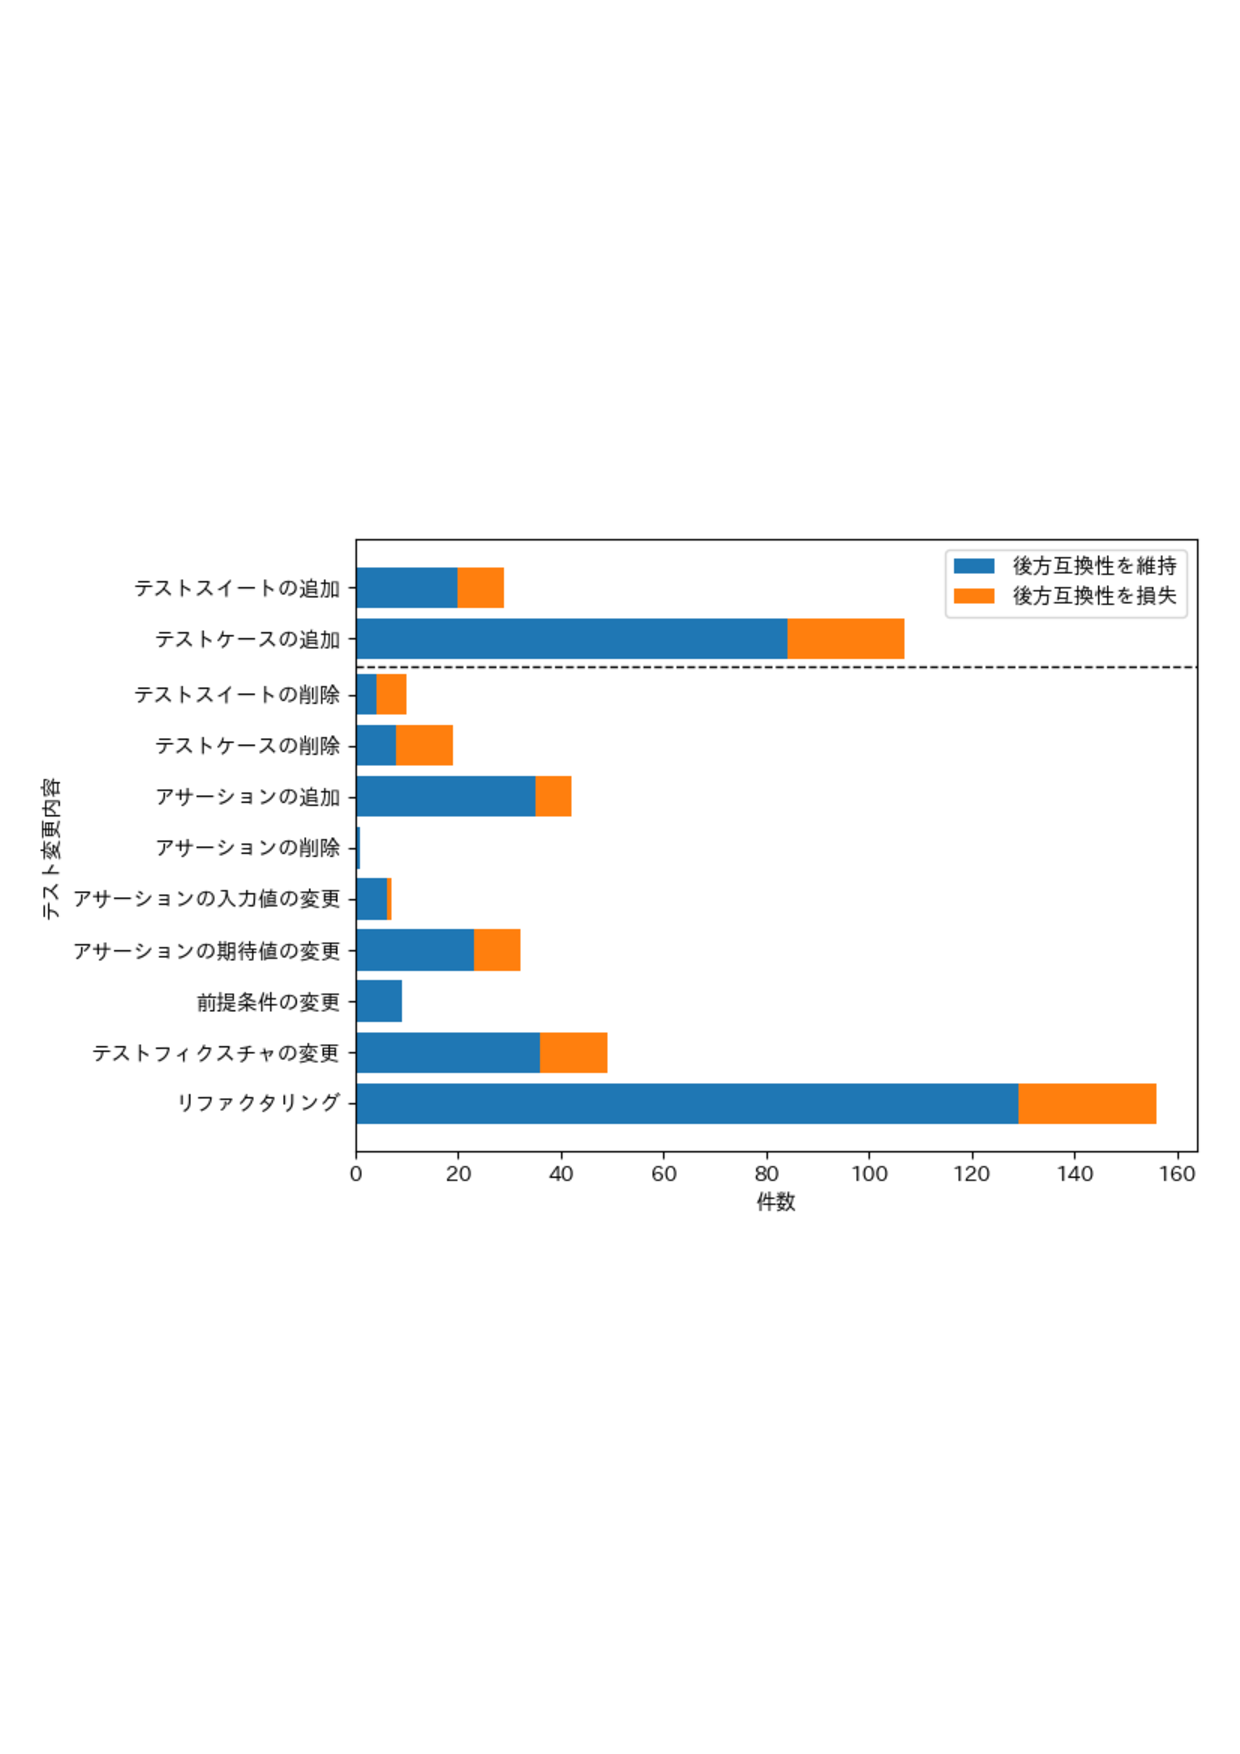
\includegraphics[width=1.0\linewidth]{fig/barh-test-pattern.pdf}
  \caption{テスト変更内容ごとの実際の後方互換性}
\end{figure}

図\ref{fig:test_pattern}は,テスト変更内容ごとの後方互換性の有無を横棒積み上げ棒グラフで示す.

テストスイートの削除,テストケースの削除は,後方互換性なしの割合が後方互換性ありの割合を上回っており,後方互換性の損失と関係のあるテストコード変更と言える.また,アサーションの削除,前提条件の変更は後方互換性を100%保っており,後方互換性の損失に関係するテストコード変更とは言えないとわかる.また,リファクタリングは件数も多くほとんどが実際に後方互換性を保っているため,従来研究の手法で誤検出となる大きな原因であるとわかる.

\section{考察}
各テスト変更内容と実際の後方互換性との関係を目視により確認し例を挙げながら考察する.

図\ref{fig:test_pattern}より,テストスイートの追加,テストケースの追加,アサーションの追加は後方互換性を損失する割合に差がない.これは,JavaScript言語の単体テストフレームワークは,テストスイート中にテストスイートを宣言することや,特定のテストケースにアサーションを複数記述することが可能で,テストスイート,テストケース,アサーションの宣言の粒度はプロジェクトに委ねられていることが挙げられる.テストスイートの削除,テストケースの削除も同様の理由で後方互換性を損失する割合に差がないと考えられる.アサーションの削除は件数が少ないため考慮しない.

\subsection{テスト追加と後方互換性の損失の関係}

\begin{figure}[t]
  \label{fig:rq1.insert-test}
  \centering
  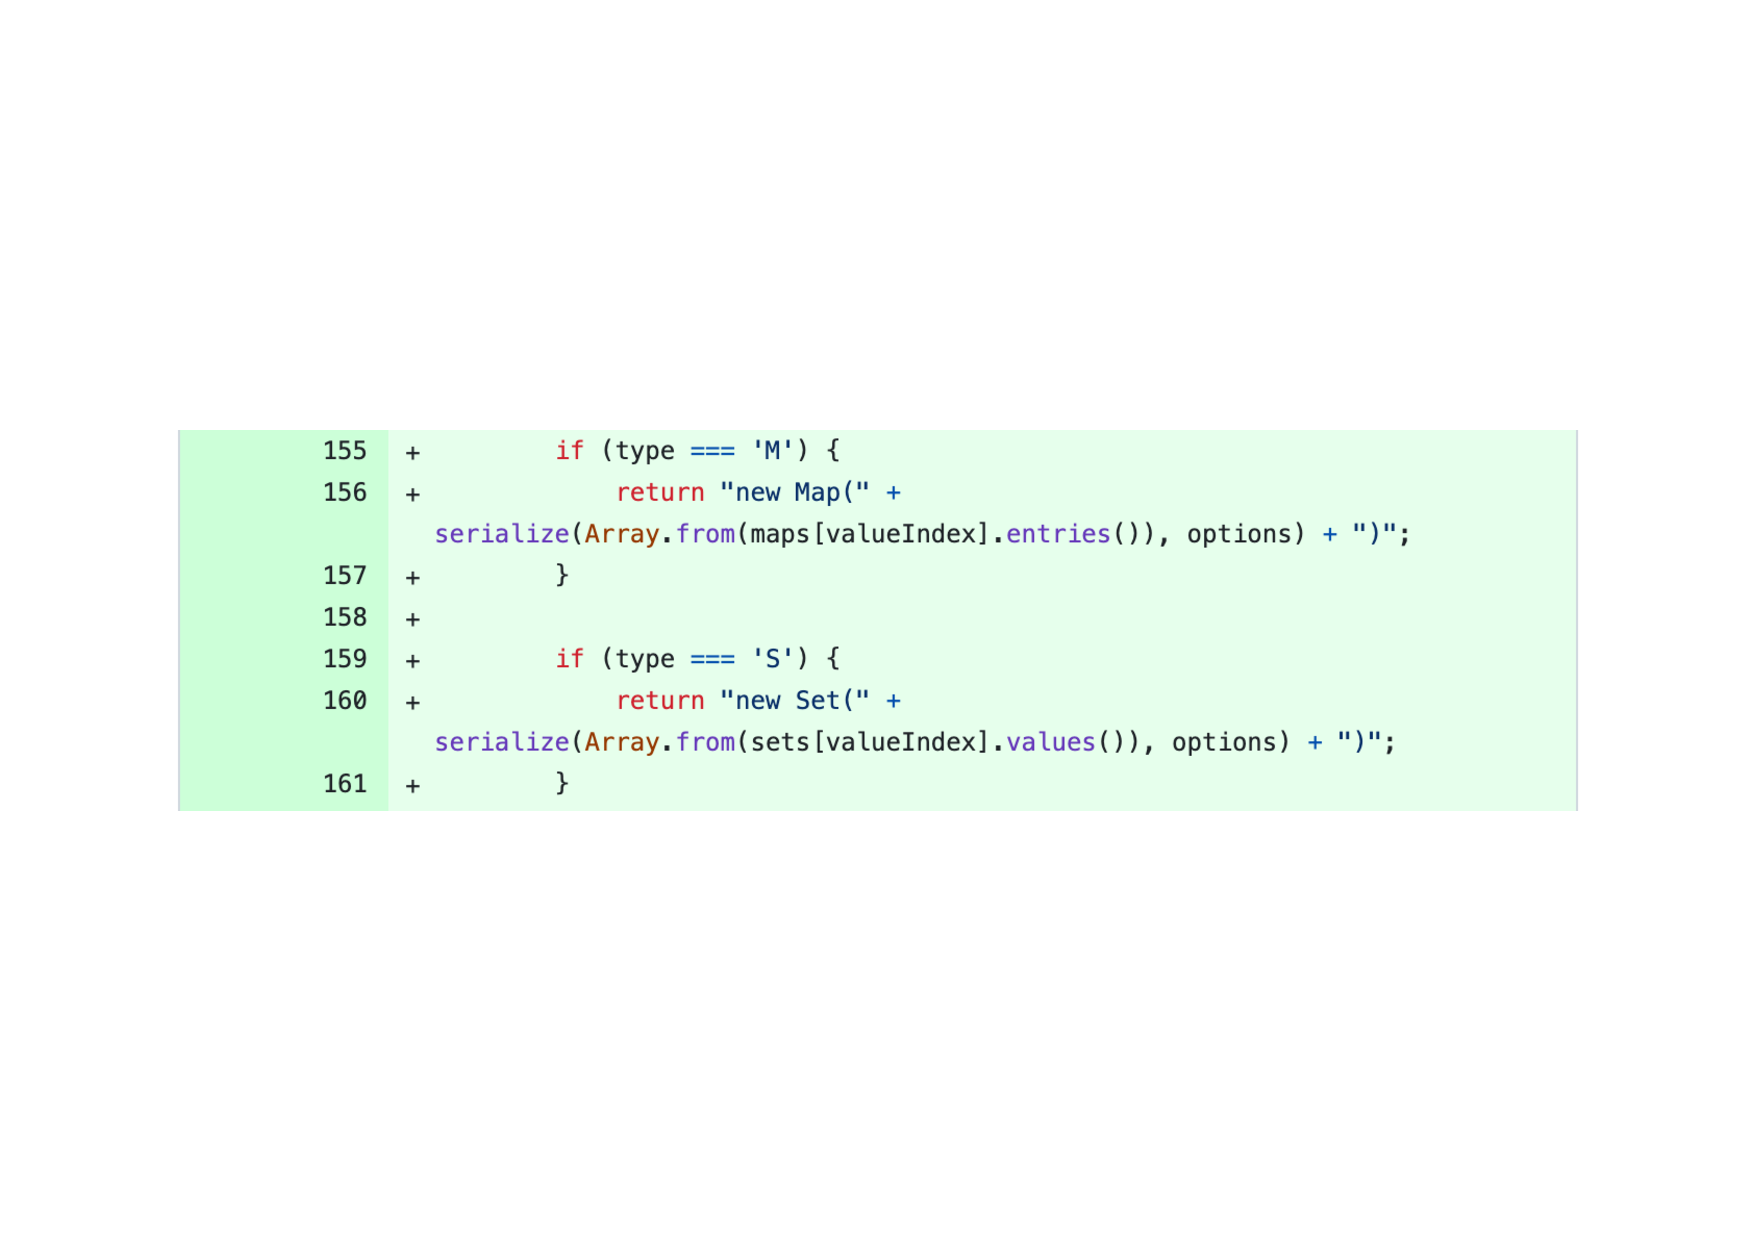
\includegraphics[width=1.0\linewidth]{fig/rq1/set-map/map.pdf}
  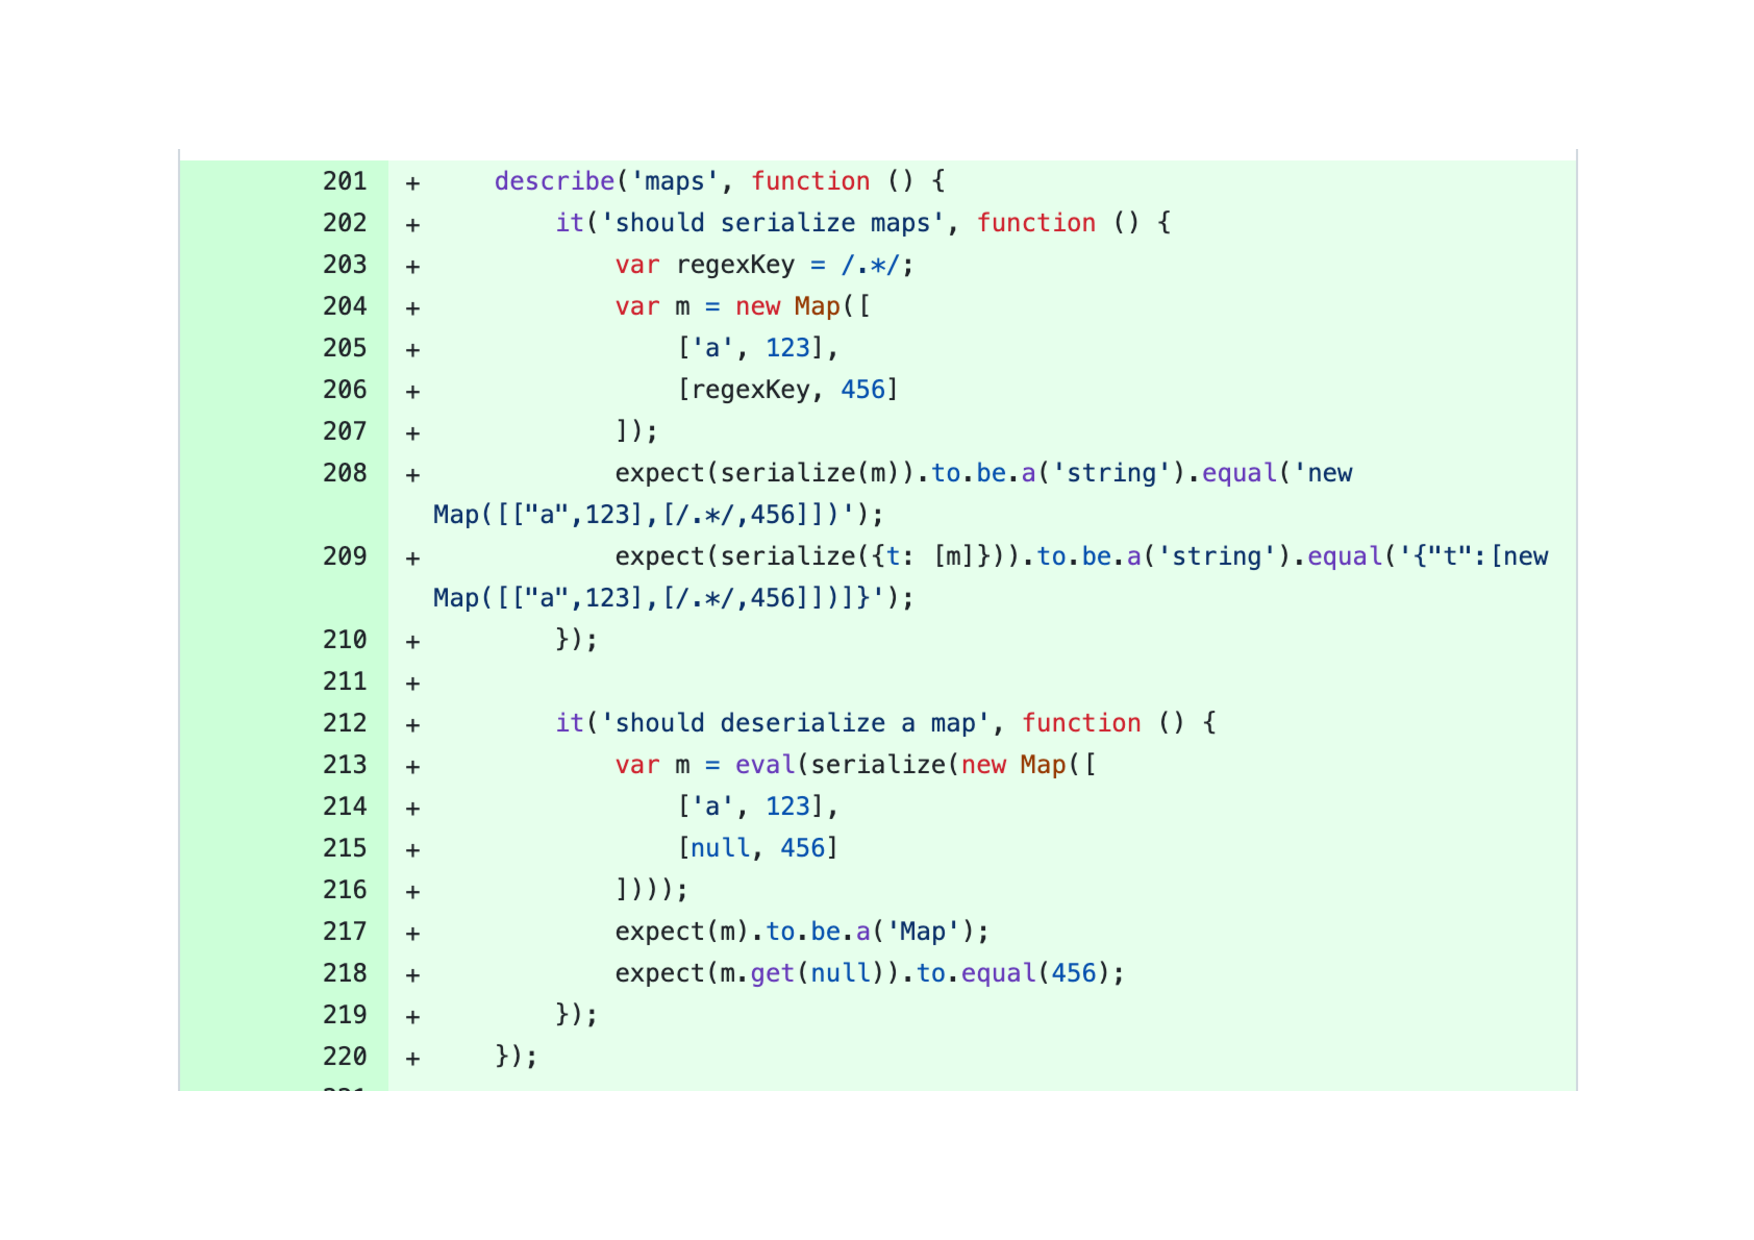
\includegraphics[width=1.0\linewidth]{fig/rq1/set-map/map.test.pdf}
  \caption{serialize-javascriptのバージョン1.6.1から1.7.0への変更}
\end{figure}

テストスイートの追加とテストケースの追加,アサーションの追加は,実際に後方互換性を保つ割合の方が高い.ただし,後方互換性の損失に伴ってテストが追加される例も存在する.後方互換性の損失に伴ってテストが追加される例として,JavaScriptオブジェクトを文字列に変換する関数を提供するライブラリserialize-javascriptのバージョン1.6.1から1.7.0への変更\footnote{\url{https://github.com/yahoo/serialize- javascript/compare/v1.6.1...v1.7.0}}を図\ref{fig:rq1.insert-test}で示す.\ref{fig:rq1.insert-test}の上部がソースコード,下部がテストコード変更内容である.

この変更では,JavaScriptでデータの集まりを扱うセット型とマップ型の入力に対し,文字列に変換する関数を適用する処理を追加している.同時に,セット型とマップ型の入力に対して文字列に正しく変換できるかを検証するテストスイートが追加されている.以前のバージョンでは,セット型とマップ型の入力に対し文字列に変換する処理がないため,文字列に変換されないことに依存しているクライアントは,バージョン更新の際に返り値が新しくなったことによる影響を受ける.このような,機能拡張による後方互換性の損失は,同時にテストが追加される場合がある.よって,機能拡張に伴うテスト追加を検出することで後方互換性の損失を捉えられると考えられる.

\subsection{テスト削除と後方互換性の損失の関係}

\begin{figure}[t]
  \label{fig:rq1.delete-test}
  \centering
  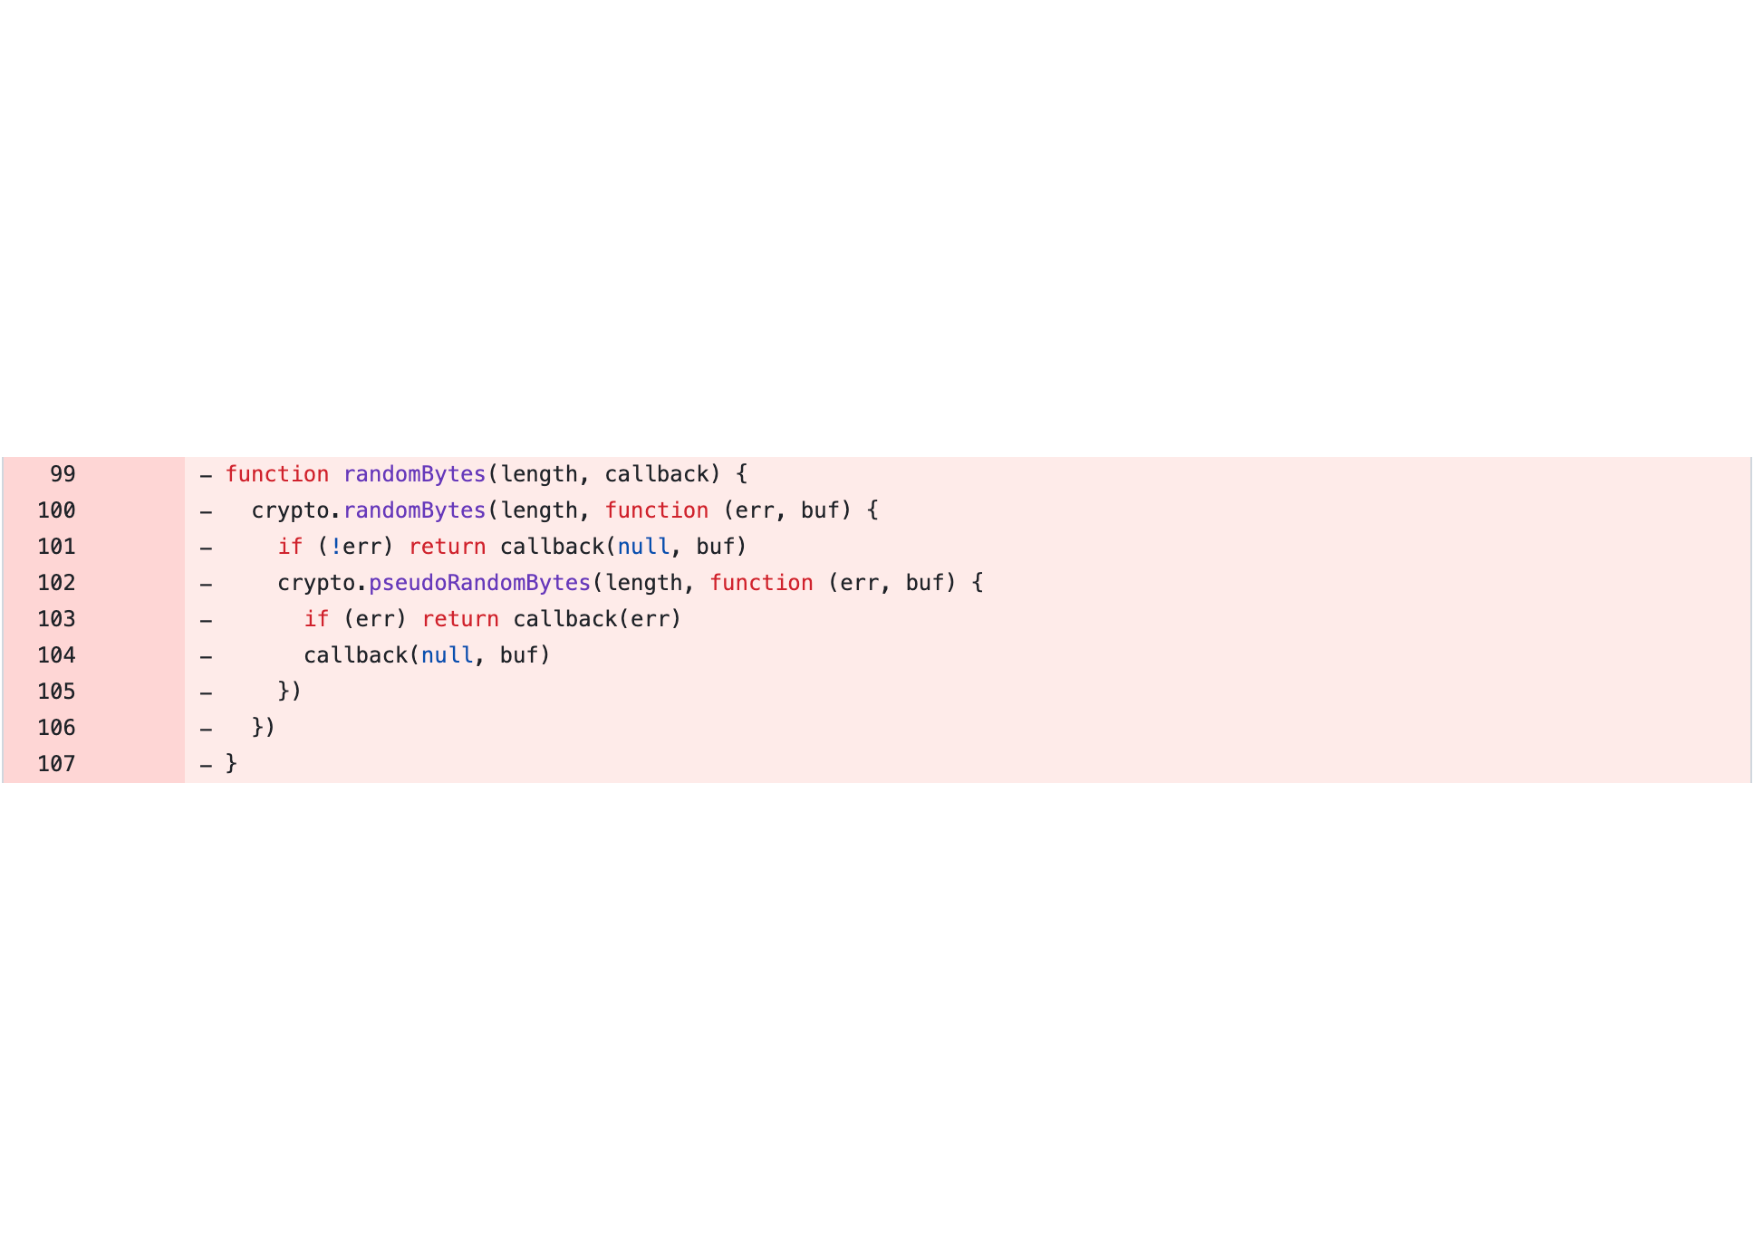
\includegraphics[width=1.0\linewidth]{fig/rq1/uuid/randomByte.pdf}
  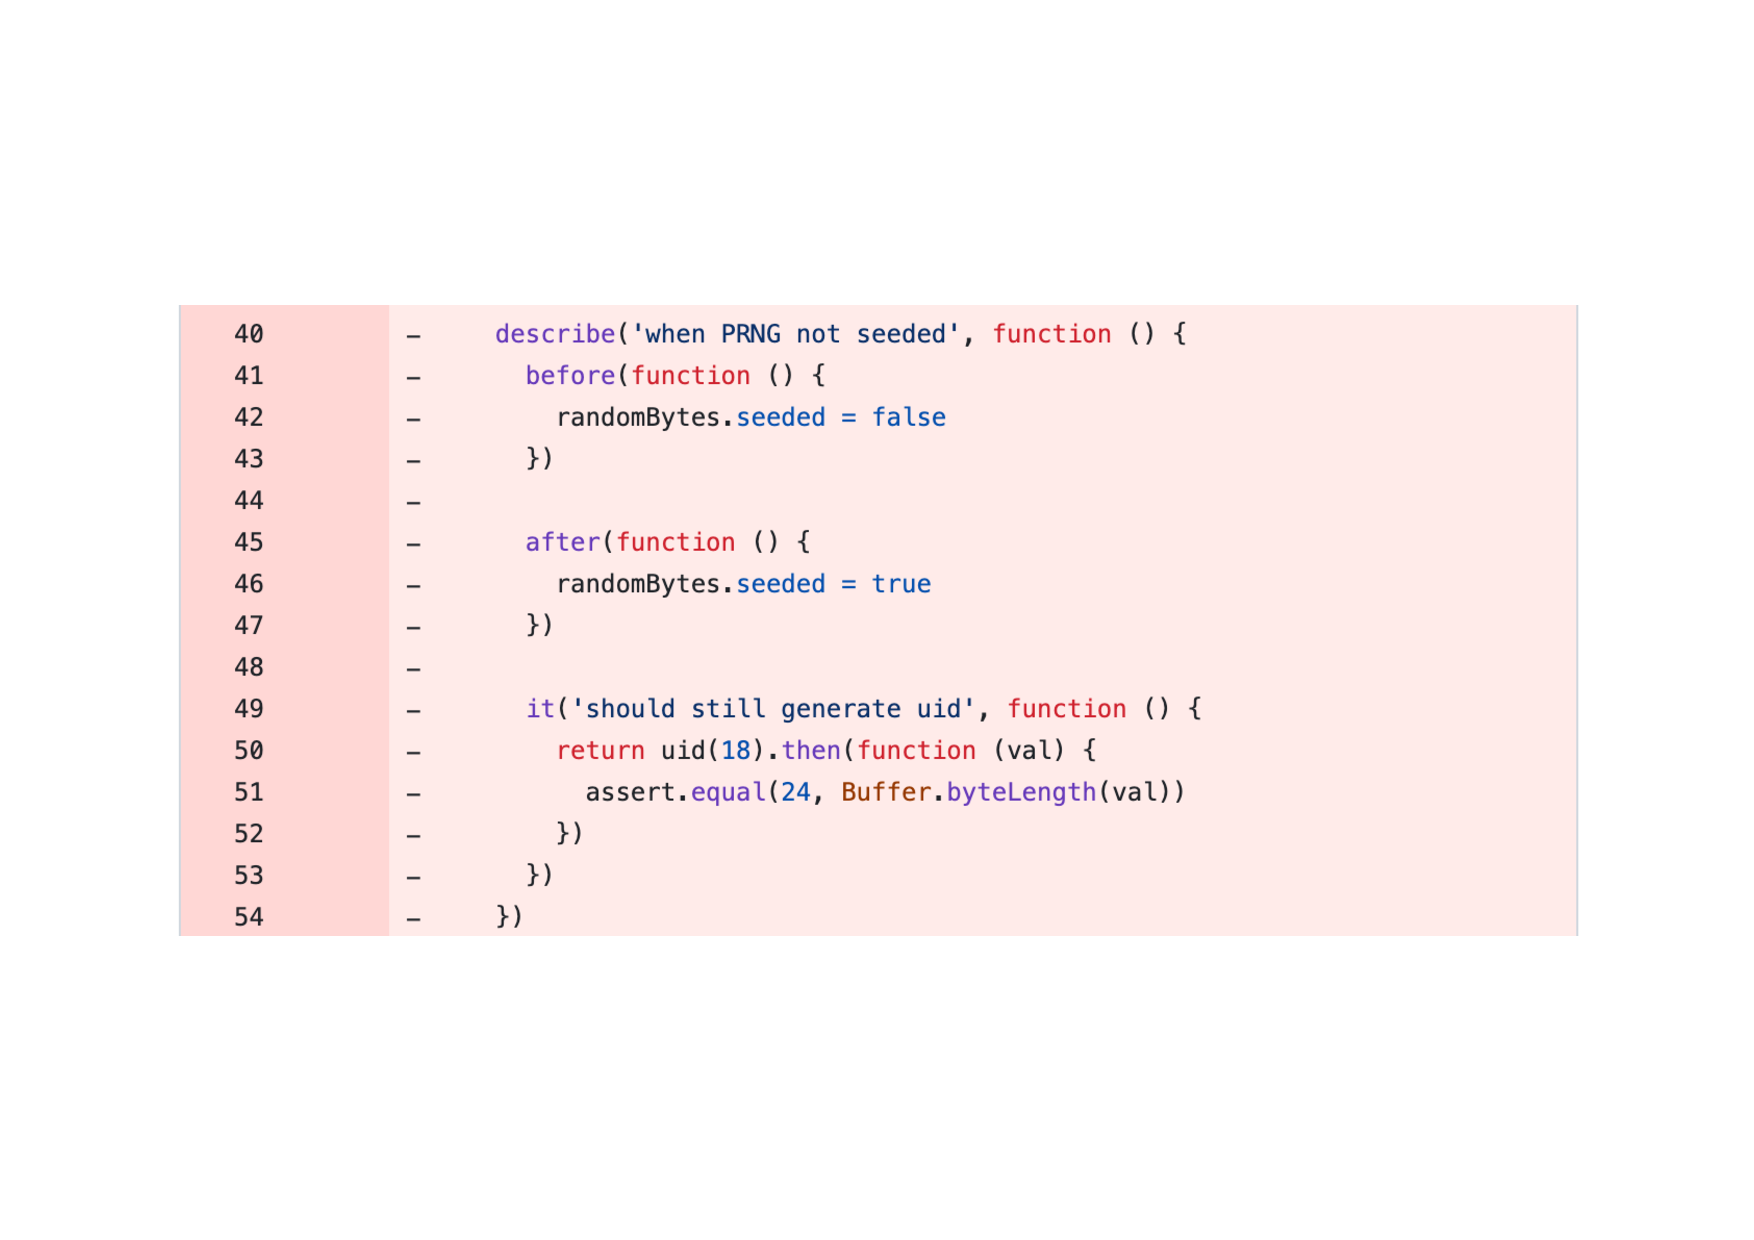
\includegraphics[width=1.0\linewidth]{fig/rq1/uuid/randomByte.test.pdf}
  \caption{uid-safeのバージョン2.0.0から2.1.0への変更}
\end{figure}

テストスイートの削除とテストケースの削除は,実際に後方互換性を損失する割合の方が高いため,テスト削除は後方互換性の損失に関係するテスト変更と言える.ただし,テストが削除されていても後方互換性の損失が検出されない場合も存在する.テストが削除されているが後方互換性の損失が検出されない例として,暗号化されたUIDを生成する関数を提供するライブラリuid-safeのバージョン2.0.0から2.1.0への変更を\footnote{\url{https://github.com/crypto-utils/uid-safe/compare/2.0.0...2.1.0}}を図\ref{fig:rq1.delete-test}で示す.図\ref{fig:rq1.delete-test}の上部がソースコード,下部がテストコード変更内容である.

この変更では,セキュリティ上の問題から,ランダムなバイト列を生成する{\verb|randomBytes|}関数を削除し,同時に{\verb|randomBytes|}の動作を検証するテストスイートを削除している.また,同バージョンで{\verb|randomBytes|}と同等のランダムなバイト列を生成するモジュールを加え,置き換えている.置き換え前後でライブラリの振る舞いが全く同じ場合,後方互換性が保たれる.また,本研究では,\ref{zissainokouhougokanseinohantei}章で述べた通り,実際の後方互換性の判定にクライアントテストを利用している.このようなモジュールに置き換える例では,振る舞いの変化が限定的になるため,クライアントテストが捉えられず後方互換性ありと誤判定されたことが考えられる.実際に影響を受けるクライアントの特定が必要になるが本研究では今後の課題とする.

\subsection{アサーションの入力値,期待値の変更と後方互換性の損失の関係}

\begin{figure}[t]
  \label{fig:rq1.change-test}
  \centering
  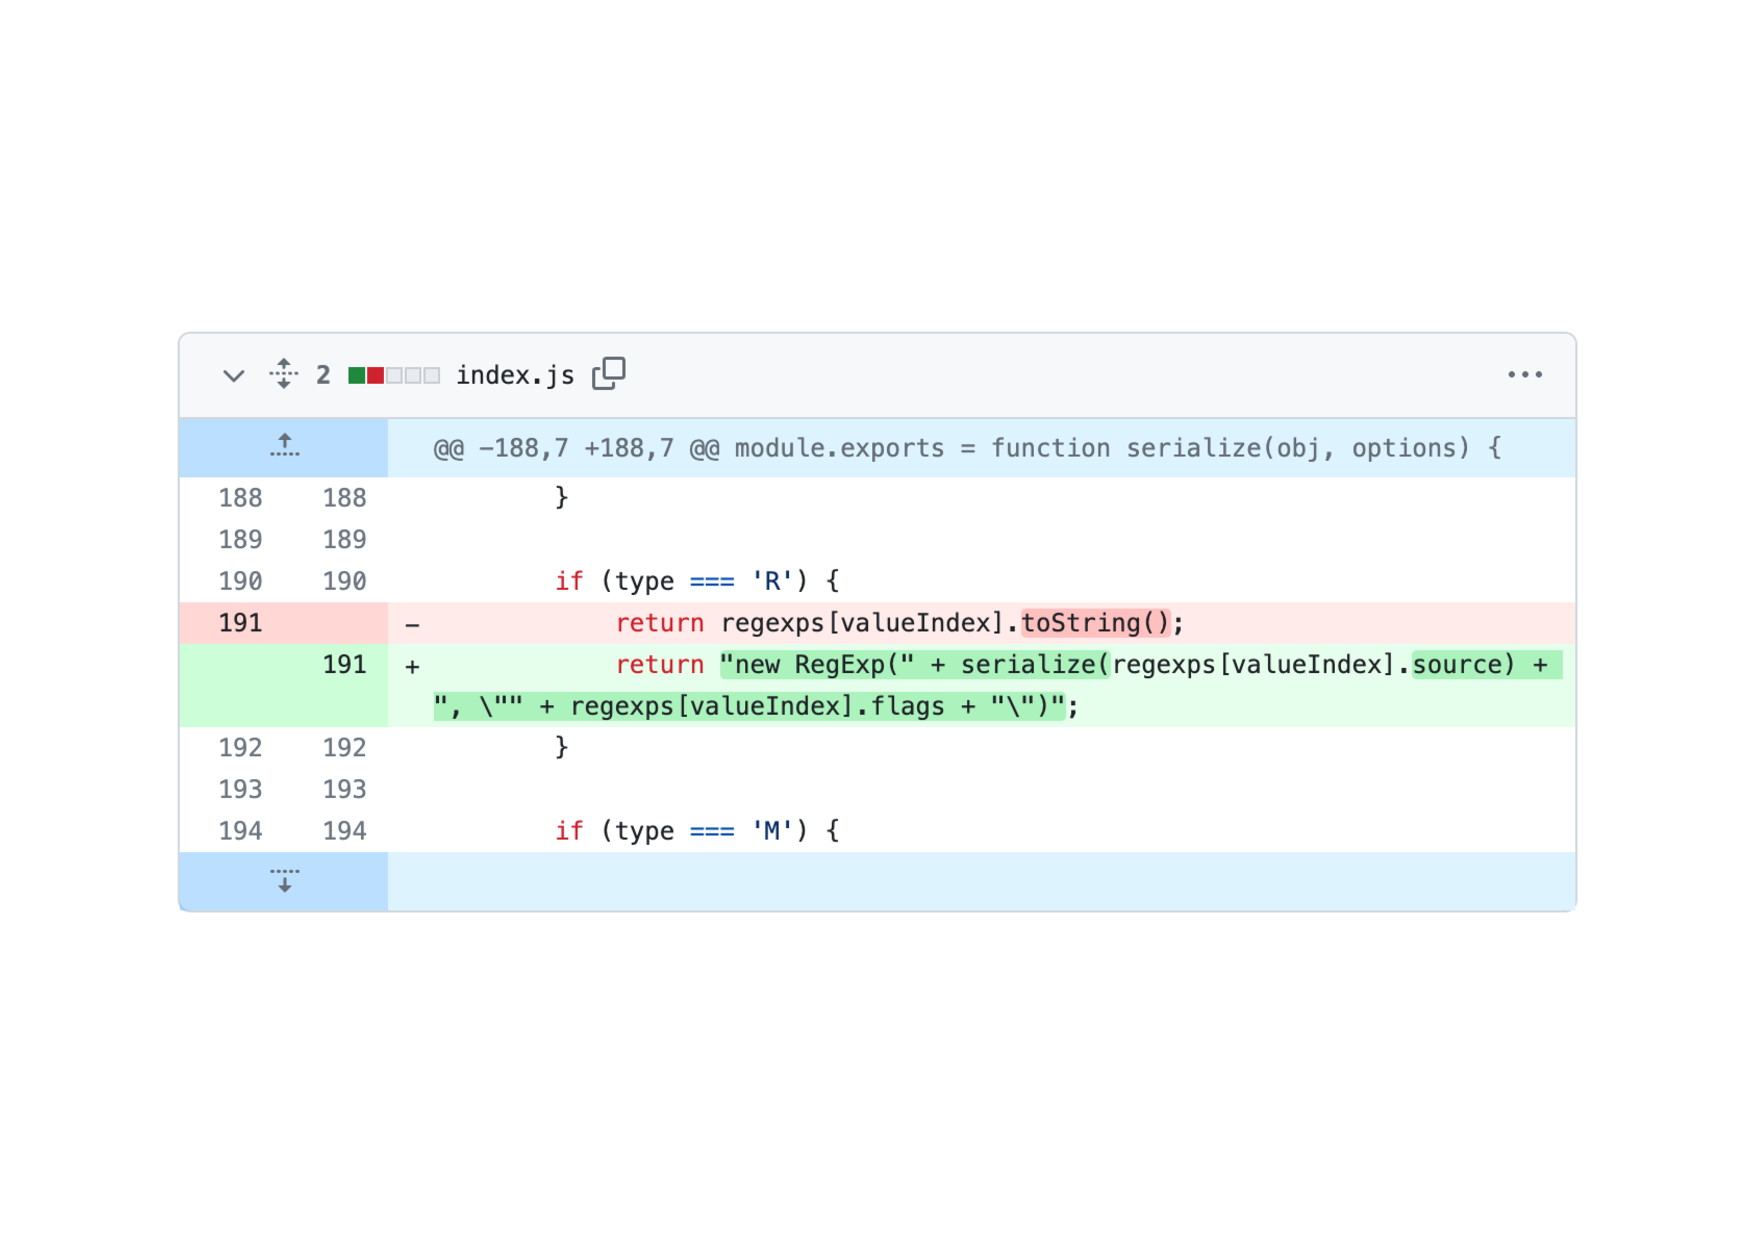
\includegraphics[width=1.0\linewidth]{fig/rq1/serialize-javascript/index.pdf}
  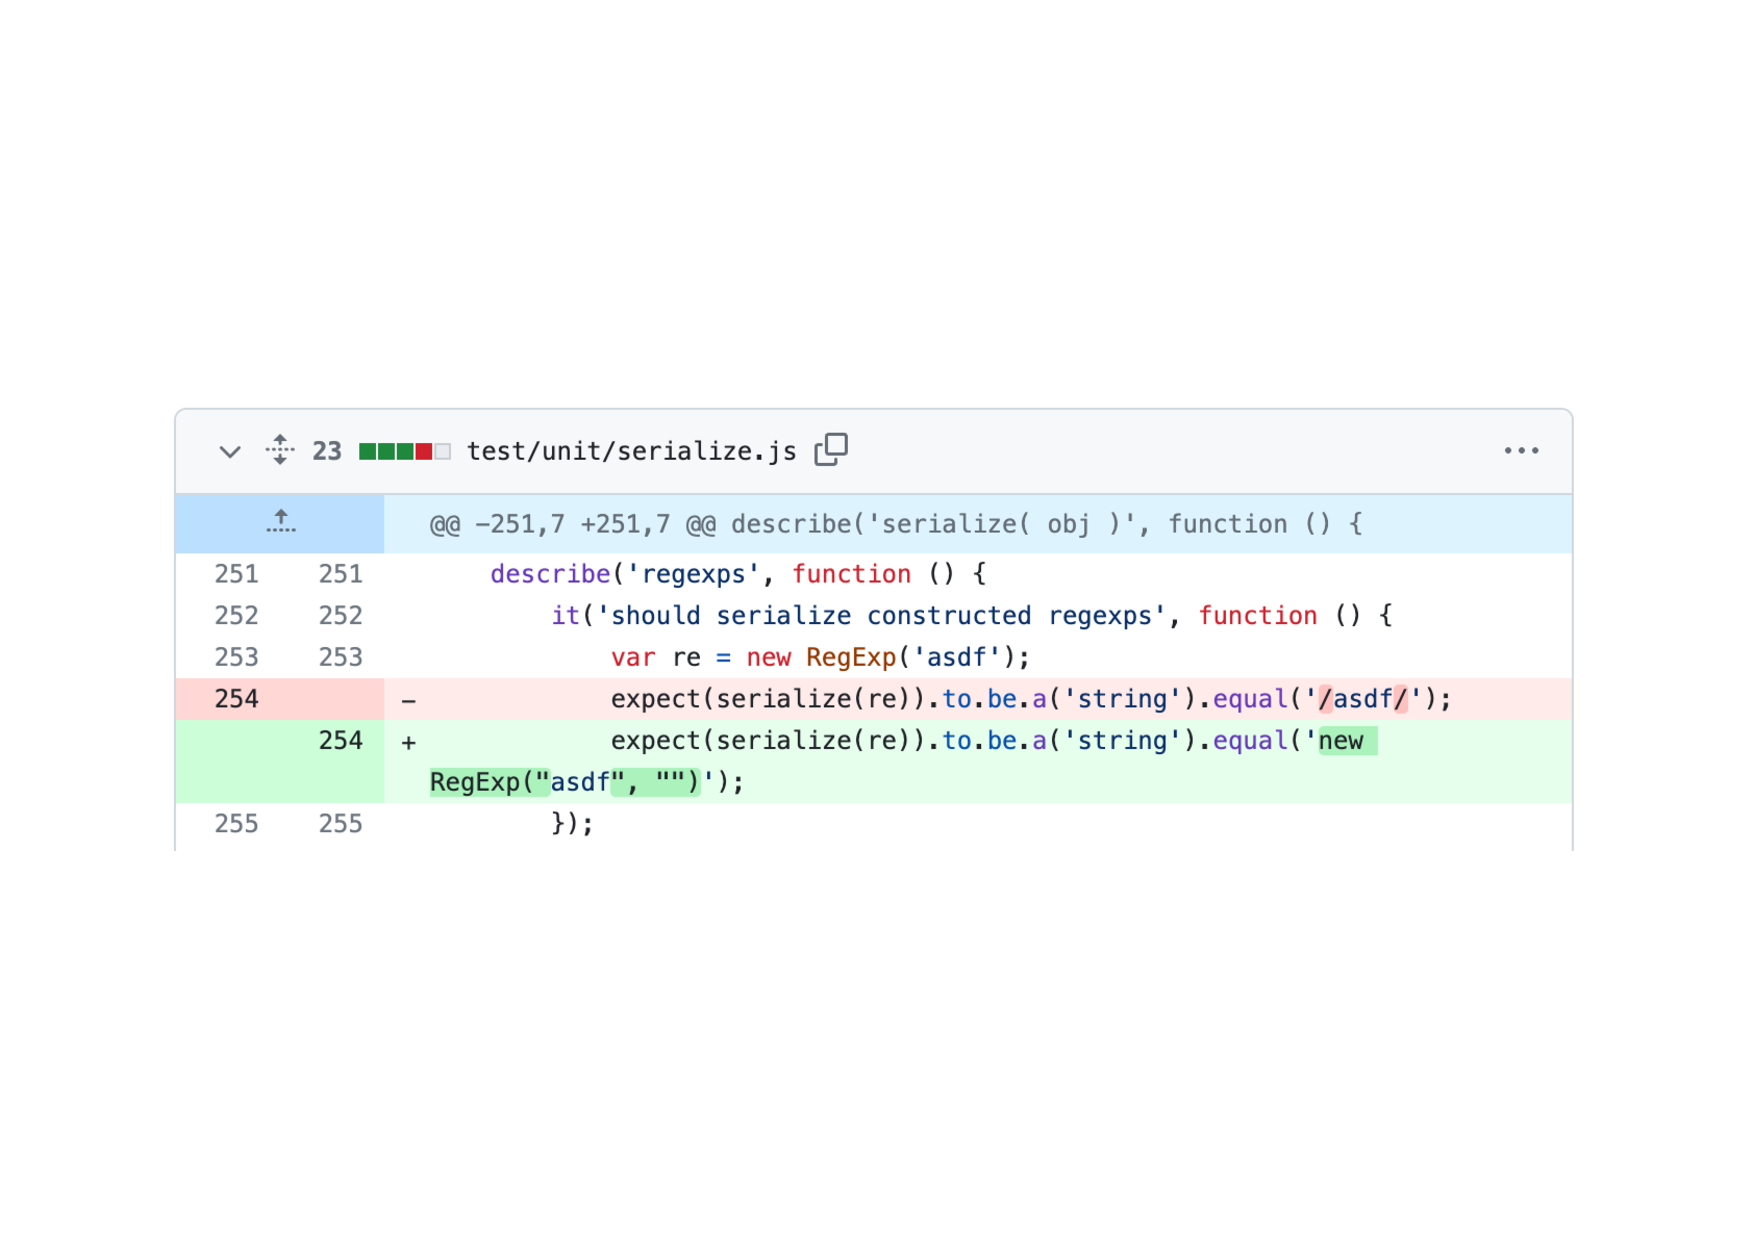
\includegraphics[width=1.0\linewidth]{fig/rq1/serialize-javascript/index.test.pdf}
  \caption{serialize-javascriptのバージョン2.1.0から2.1.1への変更}
\end{figure}

アサーションの入力値,期待値の変更は実際に後方互換性を保つ割合の方が高い.ただし,後方互換性の損失に伴ってアサーションの入力値,期待値が変更される例も存在する.後方互換性の損失に伴ってアサーションの期待値が変更される例として,serialize-javascriptのバージョン2.1.0から2.1.1への変更\footnote{\url{https://github.com/yahoo/serialize-javascript/compare/v2.1.0...v2.1.1}}を図\ref{fig:rq1.insert-test}で示す.

この変更では,セキュリティ上の問題により,正規表現に対する関数の出力が変更されている.同時に,正規表現の入力に対する返り値を検証するテストケースの期待値を変更している.よって,正規表現の入力に対して以前のバージョンでの返り値を期待するクライアントは影響を受けることがわかる.

また,後方互換性の損失に伴ってアサーションの入力値が変更される例として,CSSの色文字列を解析するライブラリcolor-stringのバージョン0.4.0から1.0.0の変更\footnote{\url{https://github.com/Qix-/color-string/compare/0.4.0...1.0.0}}では,特定の関数の使用方法が変わったことによってアサーションの入力値が変更されている.

これらの例のように,ライブラリが提供する関数の仕様変更による後方互換性の損失は,同時にアサーションの入力値や期待値が変更される場合がある.よって,仕様変更に伴うアサーションの入力値や期待値の変更を検出することで後方互換性の損失を捉えられると考えられる.

\section{まとめ}
\ref{rq1}章では,実際に後方互換性が損失した時,どのようなテスト変更が行われているかを分析した.分析により,機能拡張に伴うテスト追加,機能削除に伴うテスト削除,ライブラリが提供する関数の仕様変更に伴うアサーションの入力値,期待値の変更が後方互換性の損失に伴うテストコード変更内容であると分かった.

\chapter{RQ2:テストコード変更内容に基づく後方互換性の判定手法の有効性はどの程度か}

\section{概要}
本章では,\ref{rq1}章で述べた,後方互換性の損失に関係するテストコード変更を自動検出するツールを開発し,後方互換性の損失の検出精度を検証する.まず,抽象構文木を用いてテストコードを定義し,


% \subsubsection{テストコード内容の定義}
% JavaScriptの単体テストフレームワークとして使用される,JestやMochaの慣習に倣い,テストコード内容の定義を行う.

% \noindent\textbf{テストコードの定義:}関数呼び出しで,関数名がdescribeまたはitまたはtestであり,第一引数が文字列,第二引数が関数呼び出しのものを,テストコードとする.

% \noindent\textbf{アサーションの定義:}アサーションの記述形式はフレームワークにより異なるが,本分析では以下のように定義を行った.



\section{分析手法}

\subsection{テストコードの定義}

\subsection{変更パターンの作成}
JavaScript言語では,テストコードを書く際にフレームワークを使うことが多い.本調査では,State of JavaScript 2022\footnote{\url{https://2022.stateofjs.com/}}で紹介されている主要なテストフレームワーク13件のうち,単体テストで使われるフレームワーク5件を考慮する.

\subsection{変更パターンの検出}

\section{分析結果}

\section{考察}

\chapter{妥当性への脅威}

\section{内的妥当性}

\section{外的妥当性}

\chapter{おわりに}

\chapter*{謝辞}

% 文献を参照する場合には,論文の最後に参考文献として列挙するとともに,
% \verb|\cite|を使って,例えば,
% \begin{quote}
%   文献\cite{1390850475731067264}によれば…
% \end{quote}
% や,
% \begin{quote}
%   …である\cite{latex2e}.
% \end{quote}
% のように参照する.

% 文献の列挙には,{\tt thebibliography}環境などを用いる\footnote{使い方
%   は,この資料のソースを参照.}.

%%%%%%%%%%%%%%%%%%%%%%%%%%%%%%%%%%%%%%%%%%%%%%%%%%%%%%%%%%%%%%%%%%%%%%%%

%%
%% 謝辞
%%
%% \begin{acknowledgements}
%% 感謝します.
%% \end{acknowledgements}

%%%%%%%%%%%%%%%%%%%%%%%%%%%%%%%%%%%%%%%%%%%%%%%%%%%%%%%%%%%%%%%%%%%%%%%%

%%
%% 参考文献
%%

\bibliographystyle{junsrt}
\bibliography{thesis}

%%%%%%%%%%%%%%%%%%%%%%%%%%%%%%%%%%%%%%%%%%%%%%%%%%%%%%%%%%%%%%%%%%%%%%%%

%%
%% 付録
%%
% \appendix
% 
% \chapter{サンプルプログラム}
% 
% プログラムリストや実行結果など,本論を補足する上で必要と思われるものが
% あれば付録として付ける.
% 
% {
% \footnotesize
% \begin{verbatim}
% #include <stdio.h>
% int main(void)
% {
%     printf("Hello, World!\n");
%     return 0;
% }
% \end{verbatim}
% }

%%%%%%%%%%%%%%%%%%%%%%%%%%%%%%%%%%%%%%%%%%%%%%%%%%%%%%%%%%%%%%%%%%%%%%%%

\end{document}
